%%%%%%%%%%%%%%%%%%%%%%%%%%%%%%%%%%%%%%%%%%%%%%
%                insertmeeting
% 1) Title (something creative & funny?)
% 2) Date (MM/DD/YYYY)
% 3) Location (ex. Hagerty High School)
% 4) People/Committees Present 
% 5) Picture 
% 6) Start Time & Stop Time (ex. 12:30AM to 4:30PM)
%%%%%%%%%%%%%%%%%%%%%%%%%%%%%%%%%%%%%%%%%%%%%%
\insertmeeting 
	{Committee Day} 
	{08/23/22}
	{Hagerty High School}
	{Anouska, Jorge, Laura, Samantha}
	{Images/RobotPics/robot.jpg}
	{4:00 - 4:30}
	
\hhscommittee{General}
\noindent\hfil\rule{\textwidth}{.4pt}\hfil
\subsubsection*{Goals}
\begin{itemize}
    \item Organize team members into respective committees

\end{itemize} 

\noindent\hfil\rule{\textwidth}{.4pt}\hfil

\subsubsection*{Accomplishments}
We started off our meeting by looking at our huddle board. Our system for keeping each other updated on our goals is nice, but it took us around 15 minutes, which was particularly long. There's a lot to do in a season, so to spend so much time is a bit much. We had to manage our time efficiently, and this wasn't very efficient. However, there wasn't a lot to do just yet since Kickoff is still a few weeks out, so we ultimately decided that we would continue to update it for a while, and decide for sure once the game is revealed.

After that, there was the committees we would need to organize into. Sorting members into committees is a great way of ensuring everyone knows what their goals for the season are, and nobody ends up doing nothing. We organized a nice way of signing up in the form of a spreadsheet with every committee: Hardware, software, Multimedia, Communications, Outreach, Technical Writing, and Strategy. Members would sign up as either a major or minor contributor, and would describe how exactly they wanted to contribute. Some of us had already done this at a previous date, but we got everybody else caught up today, getting the document up to date.

Outside of committees, we also had a spreadsheet with some important contact related details, like phone number, email, grade level, etc. These will be used to ensure everybody stays up to date on the work of everyone else, and will play a large role in our success going forward.

We're starting up our FLL season soon, and we work with children at all levels. The presentations for Discover and Explore released recently, so we got them all ported over to our collective google drive for later usage. We're excited to get started with the FLL season, and plan on reviewing and editing these presentations for our purposes soon.

As a robotics team, its important to advertise ourselves to potential sponsors. The primary way of doing this is through social media. While it is the Social Media committee's job to work on these posts, we decided to brainstorm ideas collectively. We came up with a summer recap post, a kickoff post, a post for our 1st FLL meeting, some milestones we can post, our new group photo, and Team Member Takeovers, where members make a post introducing themselves to our online audience. While the ideas aren't anything out of the ordinary, it is a solid plan to start off with for the season, and will hopefully lead to a strong social media presence for the season.

\begin{figure}[htp]
\centering
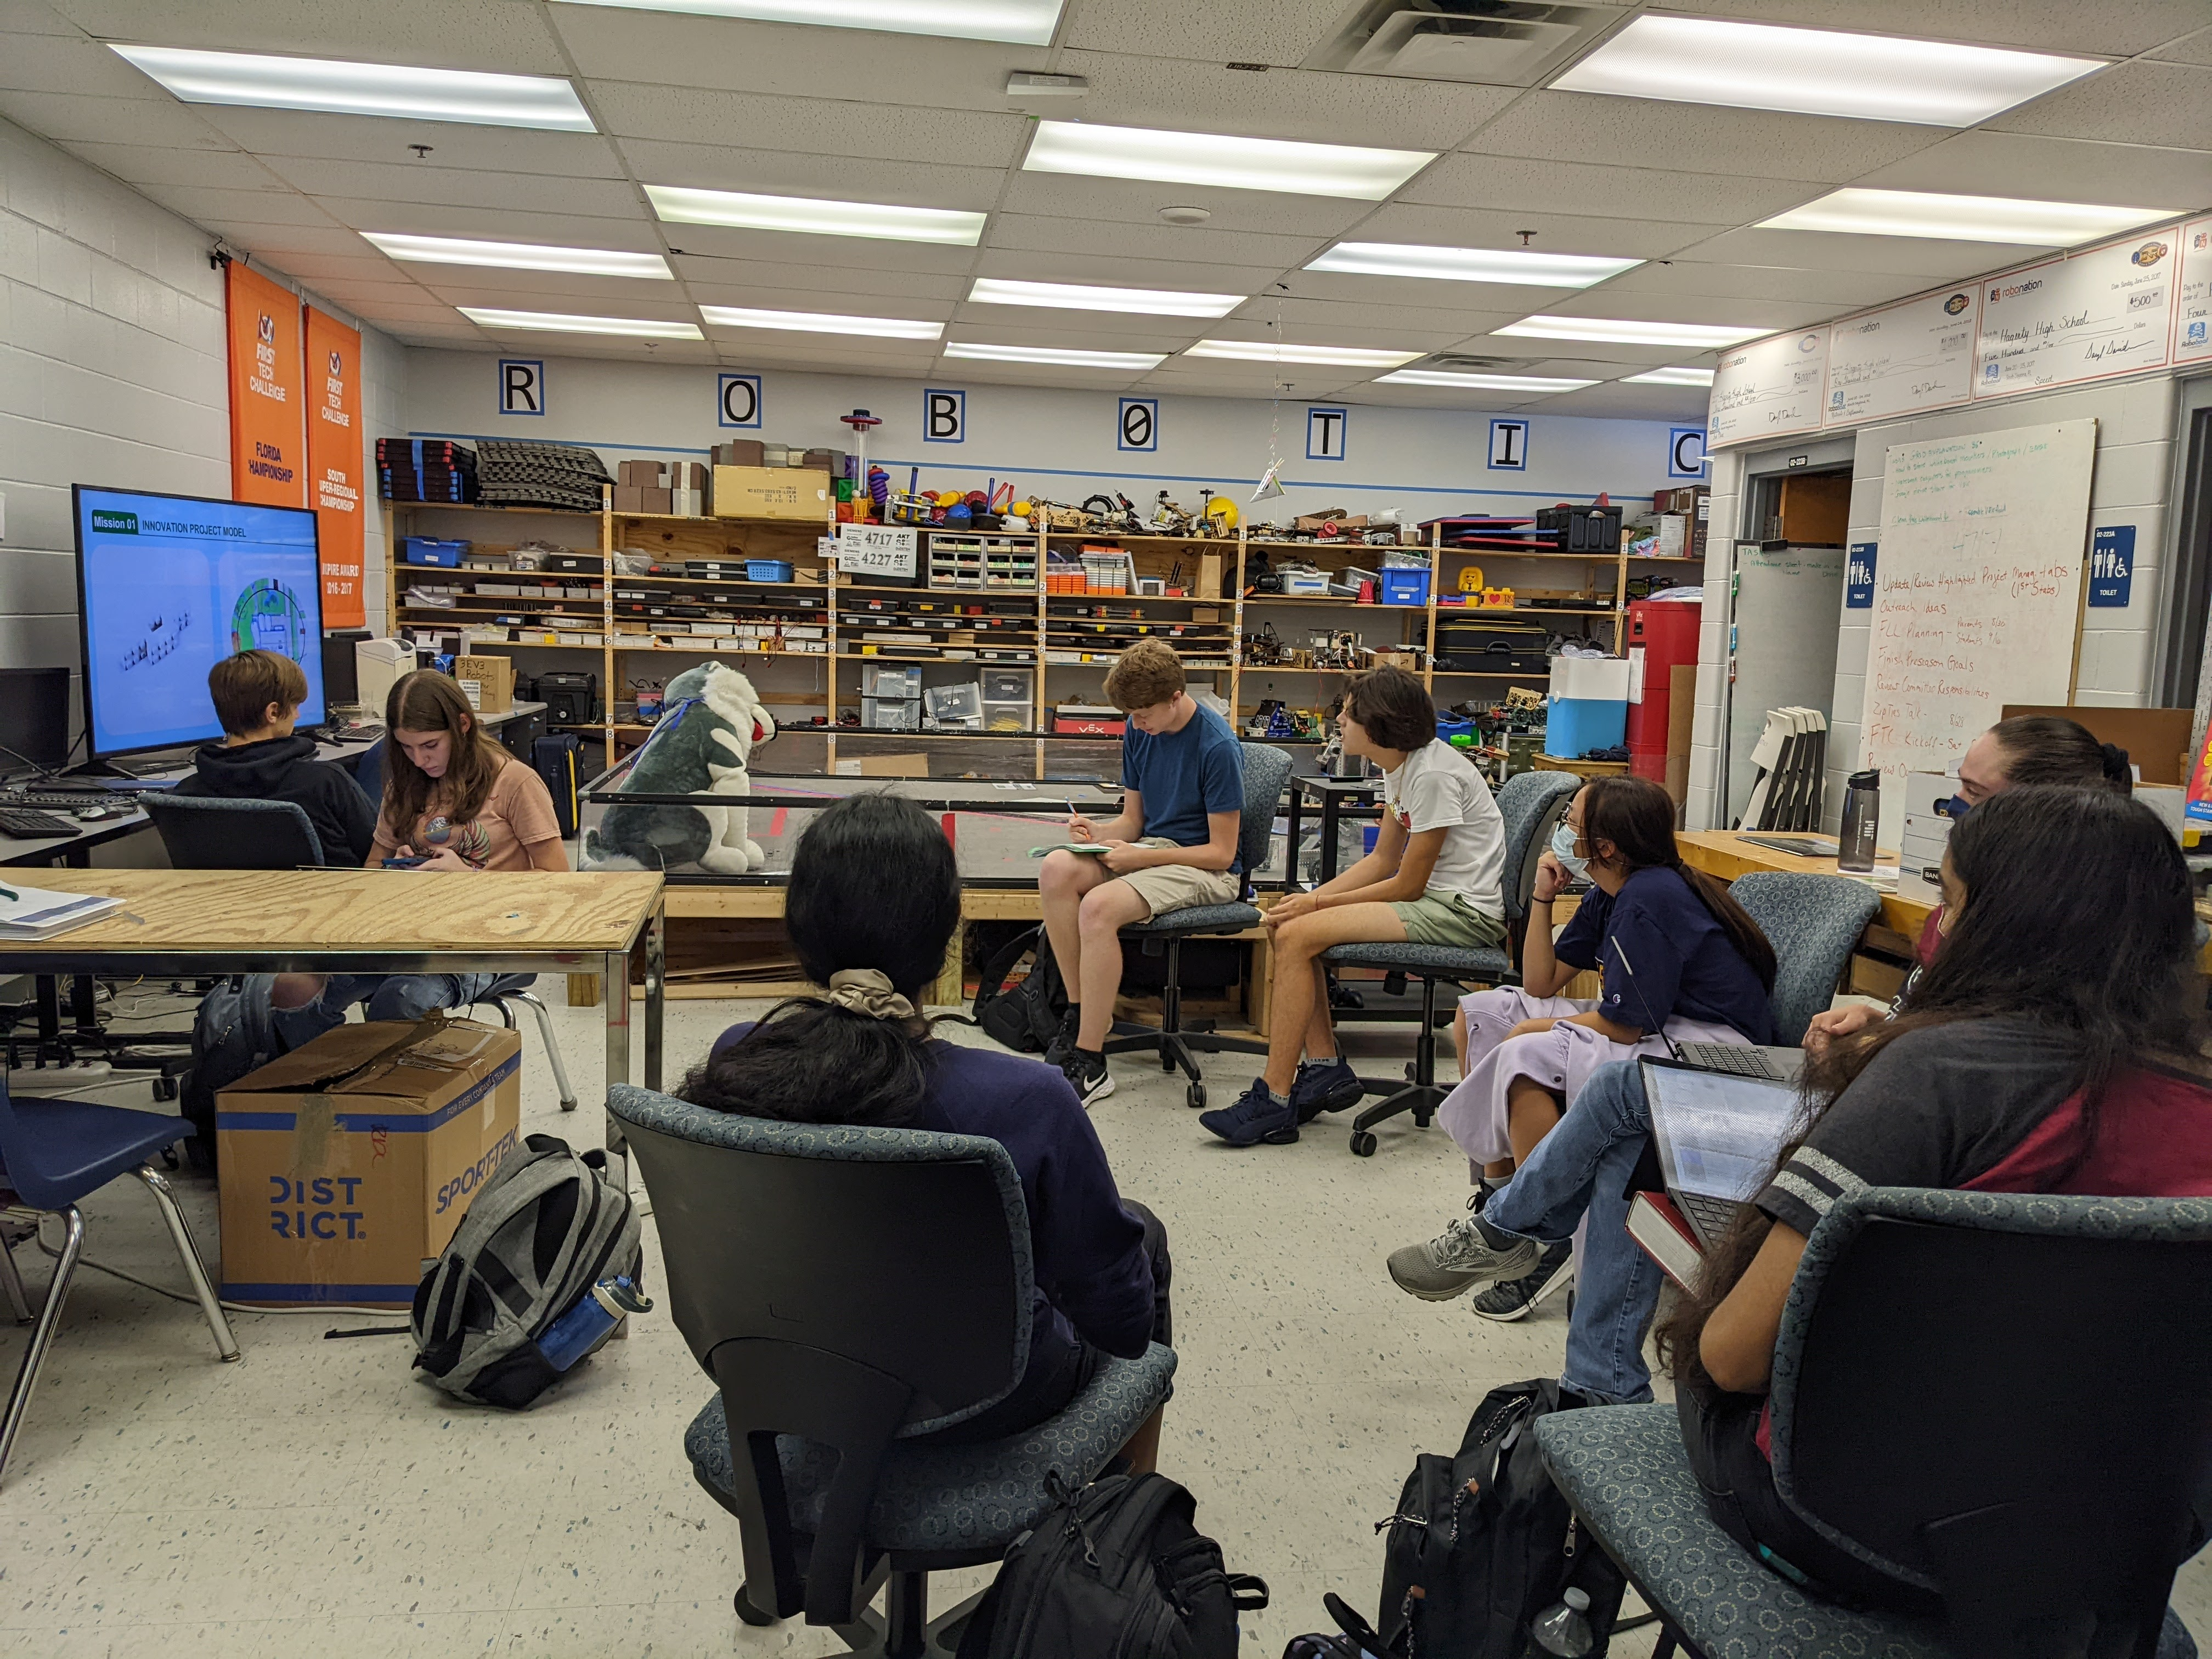
\includegraphics[width=0.9\textwidth, angle=0]{Meetings/August/08-23-22/08-23-22-meeting.jpg}
\caption{Team planning for season.}
\label{fig:082322}
\end{figure}



\whatsnext{
\begin{itemize}
    \item Plan out future outreach opportunities for the season

\end{itemize} 
}

